
\chapter{Introduction and Background}

\section{Stars}

It is common knowledge that the star closest to Earth is the Sun, and also that the Sun is yellow. It is this yellow sunlight which is interesting for some of its properties \cite{scholes2011lessons}. For instance, plants, algae, and cyanobacteria convert this light into energy via photosynthesis. In \ref{fig:firstFig} is a photo of a galaxy which contains many stars.

\begin{figure}[ht]
    \centering
	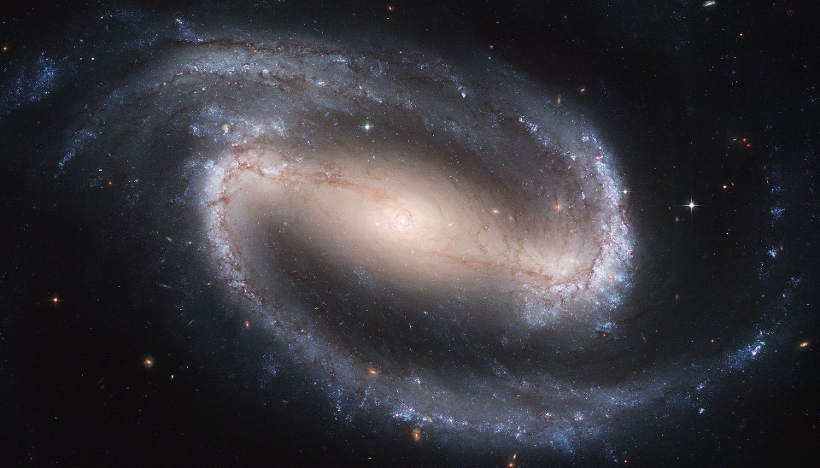
\includegraphics[width=0.85\textwidth]{figures/sampleFig1.jpg}
	\caption[Barred spiral galaxy NGC 1300]{Barred spiral galaxy NGC 1300 photographed by Hubble telescope. While the galaxy in the photo is not our sun, it does emit light, much like our sun. Image credit: NASA.}
	\label{fig:firstFig}
\end{figure}

The stars in the sky are of particular interest to the aptly named \gls{starlabs}, which in many recent experiments has shown promising results in converting this energy in a non-photoelectric sense into usable energy \cite{allen2019fast}. Interestingly, \gls{starlabs} has theorized that the famous superhero known as ``Superman'' converts the light from our sun, which grants his fantastic abilities. There are many methods in industry for converting the sun's energy (of about \SI{1000}{\watt\per\meter\squared}) into electrical energy. Some of these are highlighted in \ref{tbl:sampleTbl1}.

\begin{table}[ht]
\centering
\caption[Selected renewable energy installations]{Renewable energy installations around the world -- the energy generated at these sites is ultimately derived from the sun}
\label{tbl:sampleTbl1}
\resizebox{0.8\textwidth}{!}{%
\begin{tabular}{llll}
\hline
installation & type & capacity (GW) & location \\ \hline
Longyangxia Dam & photovoltaic & 0.85 & China \\
Gansu Wind Farm & wind & 6 & China \\
Sihwa Lake & tidal & 0.254 & South Korea \\ \hline
\end{tabular}%
}
\end{table}